\documentclass[10pt,letterpaper]{article}
%----------------------------------------------------------------------------------------
%	PACKAGES AND OTHER DOCUMENT CONFIGURATIONS
%----------------------------------------------------------------------------------------

\usepackage{amsmath,amsfonts,stmaryrd,amssymb} % Math packages
\usepackage{amsfonts}
\usepackage{float}
\usepackage{enumerate} % Custom item numbers for enumerations
\usepackage{mathtools}
\usepackage{mathrsfs}
\usepackage{commath}
\usepackage[ruled]{algorithm2e} % Algorithms
\newtheorem{proof}{PROOF}
\usepackage[framemethod=tikz]{mdframed} % Allows defining custom boxed/framed environments

\usepackage[T1]{fontenc}
\usepackage{bigfoot} % to allow verbatim in footnote
\usepackage{python}
\usepackage{graphicx}
\usepackage{geometry}
% \userpackage{pdfpages}

\usepackage{lipsum}

\newcommand{\overbar}[1]{\mkern 1.5mu\overline{\mkern-1.5mu#1\mkern-1.5mu}\mkern 1.5mu}
\geometry{letterpaper, portrait, margin=1.5cm}




\title{ECE421 Introduction to Machine Learning \\
    Assignment \#3 \\
    Unsupervised Learning and Probabilistic Models}
\date{Mar 2019}
\author{
  Yan, Xuanming\\
  \texttt{xuanming.yan@mail.utoronto.ca} \\
  1001175382 \\
  Contribution: 50\%
  \and
  Wang, Chu Qing\\
  \texttt{eliza.wang@mail.utoronto.ca} \\
  1001303573\\
  Contribution: 50\%
} % Author name and email address
\usepackage[utf8]{inputenc}
 
\usepackage{listings}
\usepackage{color}
 
\definecolor{codegreen}{rgb}{0,0.6,0}
\definecolor{codegray}{rgb}{0.5,0.5,0.5}
\definecolor{codepurple}{rgb}{0.58,0,0.82}
\definecolor{backcolour}{rgb}{0.95,0.95,0.92}
 
\lstdefinestyle{mystyle}{
    backgroundcolor=\color{backcolour},   
    commentstyle=\color{codegreen},
    keywordstyle=\color{magenta},
    numberstyle=\tiny\color{codegray},
    stringstyle=\color{codepurple},
    basicstyle=\footnotesize,
    breakatwhitespace=false,         
    breaklines=true,                 
    captionpos=b,                    
    keepspaces=true,                 
    numbers=left,                    
    numbersep=5pt,                  
    showspaces=false,                
    showstringspaces=false,
    showtabs=false,                  
    tabsize=2
}
 
\lstset{style=mystyle}

\begin{document}
% 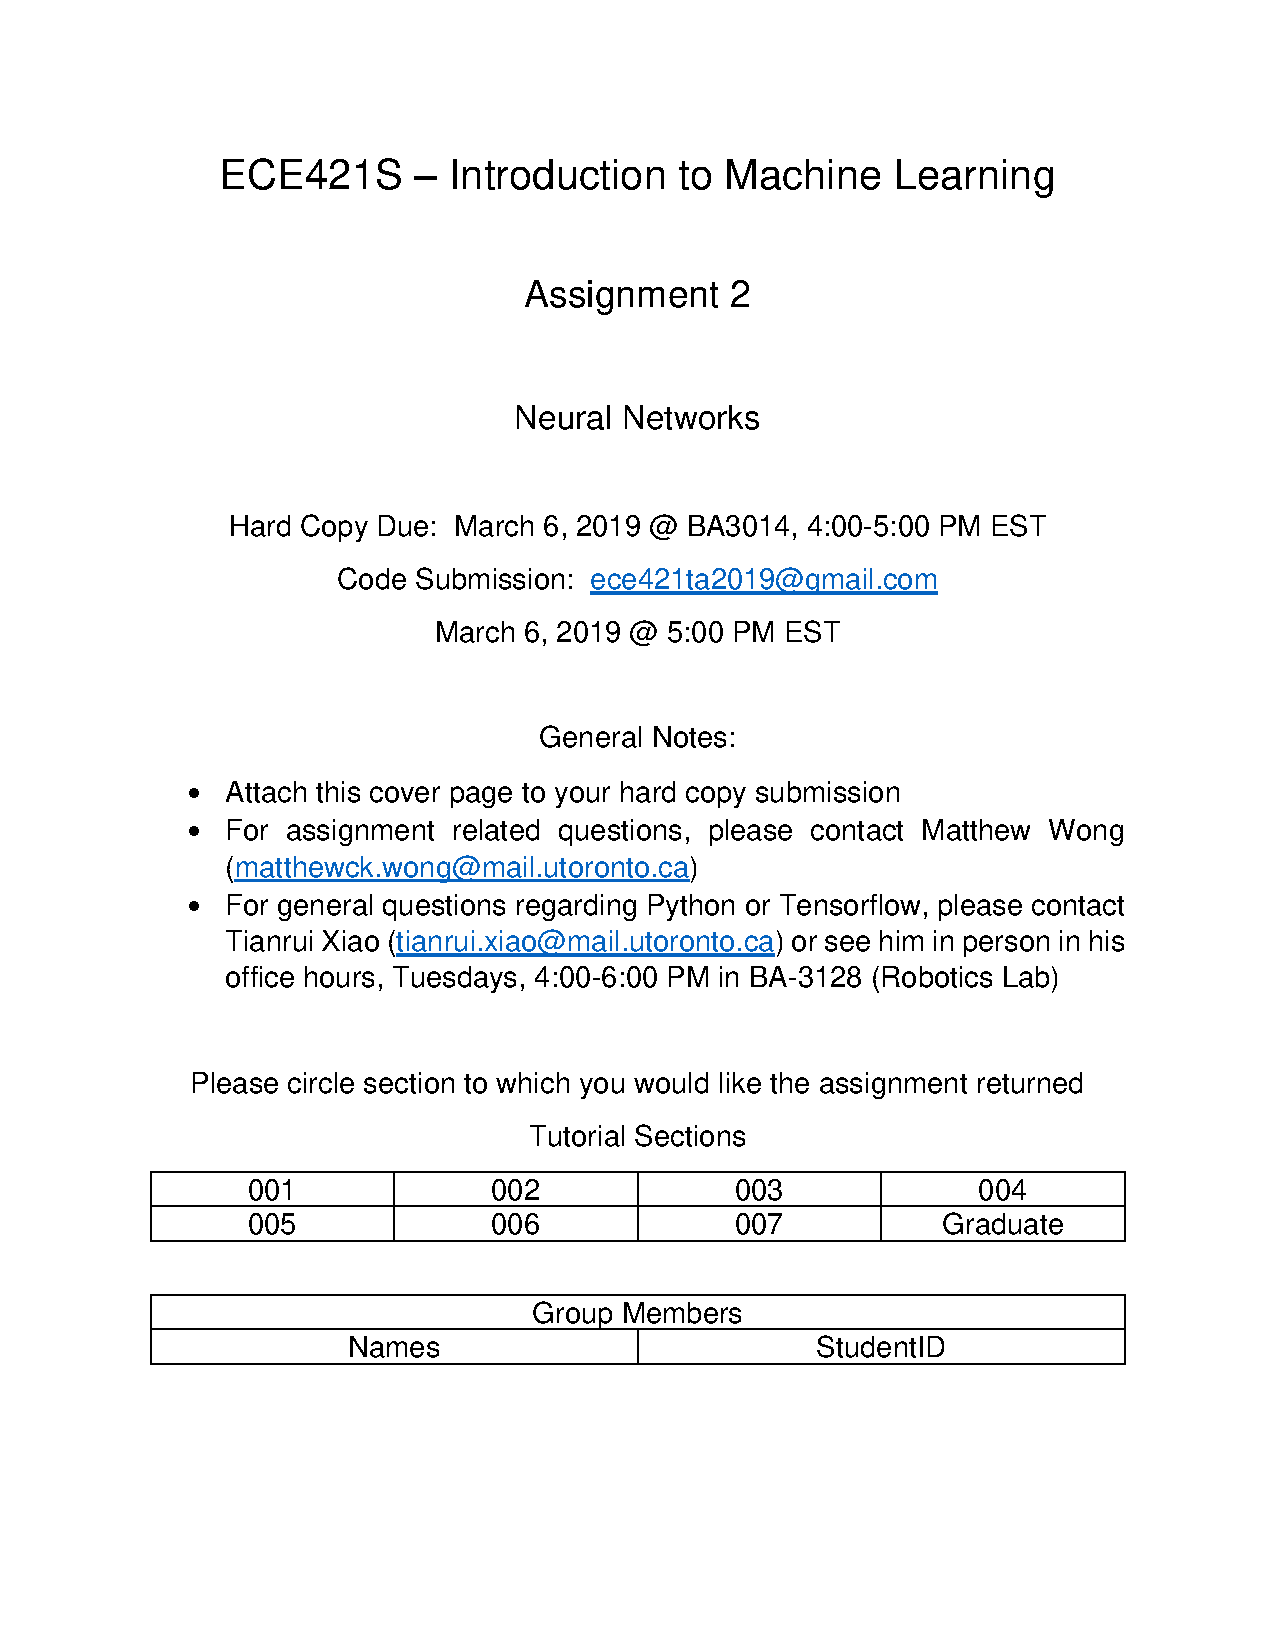
\includegraphics[width=1\linewidth]{a2cover.pdf}


\maketitle % Print the title

\section{K-means}


\subsection{}
\qquad We had implemented the distance function by using pairwise squared distance between $X$ and $MU$, and the helper function "assign\_data" returns a list of indexes for every $x$ to its closest K-mean. We chose $200$ iterations to train the data, since we could see obvious decay in loss.\\

First, we randomly initialize k centers using Gaussian distribution, with $stddev = 1$. $ \mu^{k} \in {\rm I\!R}^{D} $. Then Assign each point $k \in \{1,…K\}$ to nearest center: $C^{(t)}(n) = argmin _{k = 1}^{K}\left\| \textbf{x}_n - \mu_{k} \right\|_2^2$. Finally, update $\mu_i$, let it becomes new centroid. 
\begin{figure}[H]
\centering

  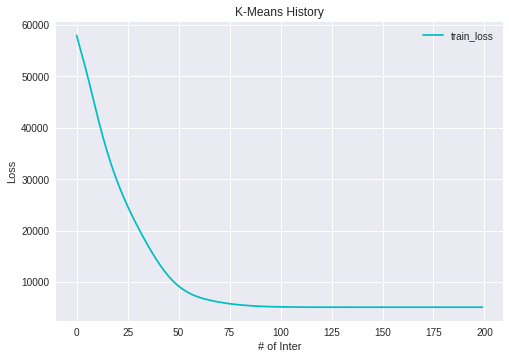
\includegraphics[width=.42\linewidth]{imgs/download.png}
  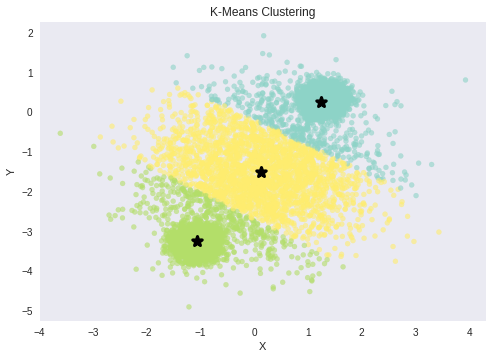
\includegraphics[width=.42\linewidth]{imgs/p1_1_2.png}
  \caption{K-means when $K=3$. Losses vs Iterations}

\end{figure}

 \lstinputlisting[language=python, caption = K-means uisng Adam optimizer]{functions/starter_kmeans.py}
\subsection{}

\qquad By looking at table 1 below, the percentage of data in each clusters are balanced up to $k=3$, from $K=4$ and onward, there exists unbalanced percentage data in each clusters, some clusters has much more data accumulated than others, therefore $k=3$ would be the best choice.\\

\begin{table}[H]
\centering
{\small

\begin{tabular}{cccccc}
\hline
 & Class 1  & Class 2      & Class 3 & Class 4 & Class 5\\ \hline
K = 1 & 100\%  & 0 & 0 & 0 & 0\\ 
K = 2 & 49.53\% & 50.47\% & 0 & 0 & 0\\ 
K = 3 & 23.81\% & 38.06\% & 38.13\% & 0 & 0\\
K = 4 & 12.03\% & 13.53\% & 37.13\% & 37.31\% & 0 \\
K = 5 & 11.07\% & 7.63\% & 37.04\% & 7.55\% & 36.71\% \\ \hline
\end{tabular}
}
\vspace{-0.2cm}
\caption{Percentage of the data points belonging to each of the K clusters.}
\label{tab:Number of hidden units}
\vspace{-0.4cm}
\end{table}


\begin{figure}[H]
\centering

  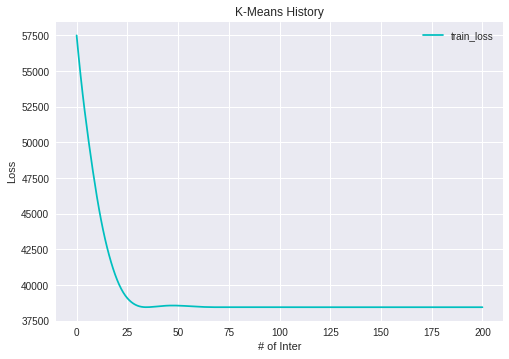
\includegraphics[width=.42\linewidth]{imgs/1_2_k1l.png}
  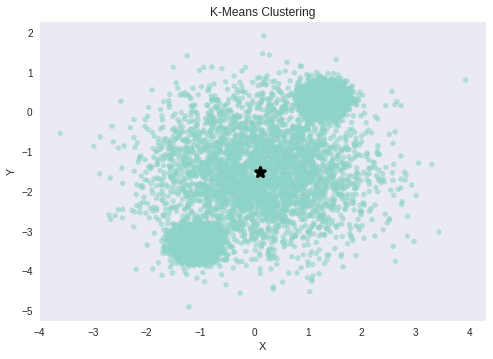
\includegraphics[width=.42\linewidth]{imgs/1_2_k1p.png}
  \caption{K-means when $K=1$. Losses vs Iterations}
  

\end{figure}

\begin{figure}[H]
\centering

  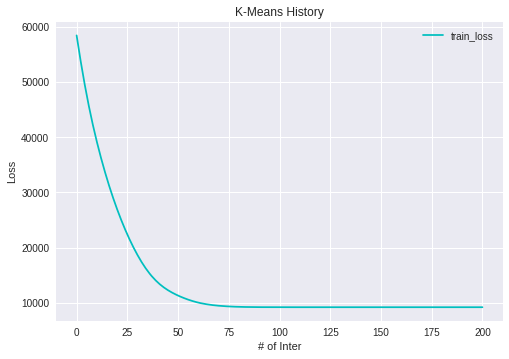
\includegraphics[width=.42\linewidth]{imgs/1_2_k2l.png}
  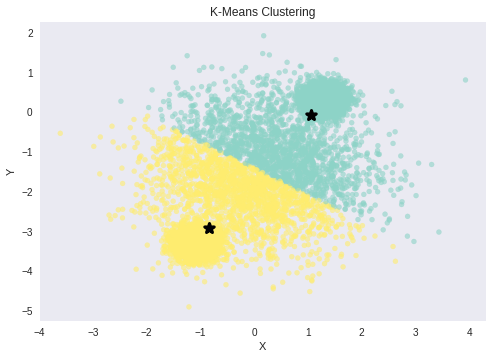
\includegraphics[width=.42\linewidth]{imgs/1_2_k2p.png}
  \caption{K-means when $K=2$. Losses vs Iterations}
  

\end{figure}

\begin{figure}[H]
\centering

  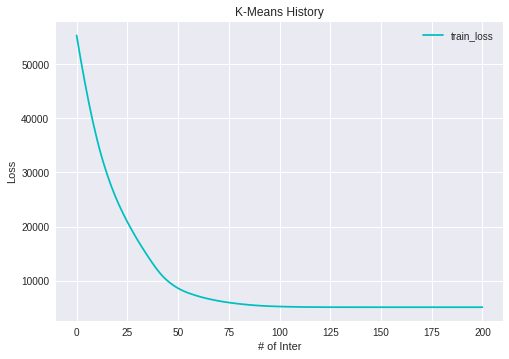
\includegraphics[width=.42\linewidth]{imgs/1_2_k3l.png}
  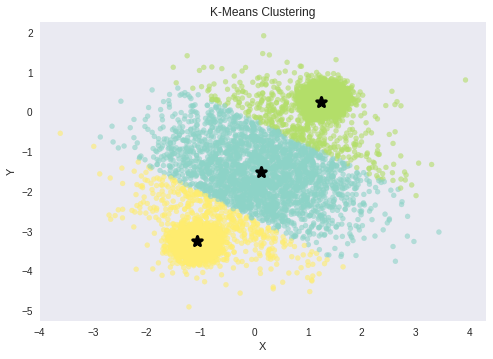
\includegraphics[width=.42\linewidth]{imgs/1_2_k3p.png}
  \caption{K-means when $K=3$. Losses vs Iterations}
  

\end{figure}

\begin{figure}[H]
\centering

  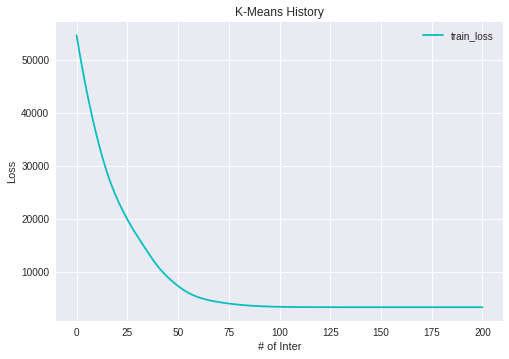
\includegraphics[width=.42\linewidth]{imgs/1_2_k4l.png}
  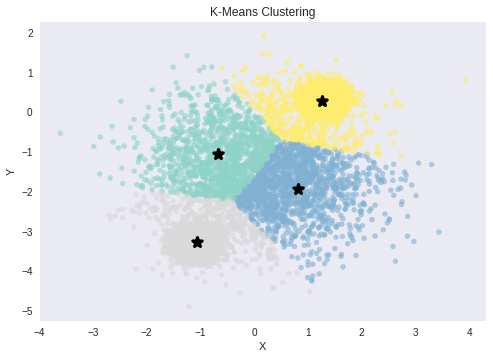
\includegraphics[width=.42\linewidth]{imgs/1_2_k4p.png}
  \caption{K-means when $K=4$. Losses vs Iterations}
  

\end{figure}

\begin{figure}[H]
\centering

  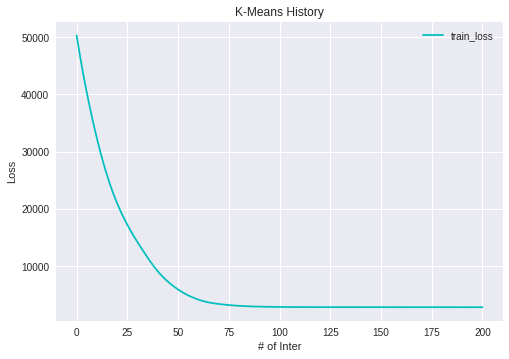
\includegraphics[width=.42\linewidth]{imgs/1_2_k5l.png}
  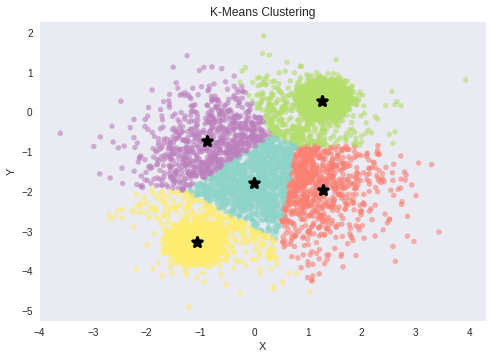
\includegraphics[width=.42\linewidth]{imgs/1_2_k5p.png}
  \caption{K-means when $K=5$. Losses vs Iterations}
  
\end{figure}



\subsection{}

\qquad We cannot draw conclusion by only looking the the loss for different cluster size, since more clusters will always gives us smaller loss value, if number of k = number of data, we can even get loss equals to zero. Therefore, instead of looking at the actual loss values, we can look at the trend of change in loss values as shown in figure 7. We notice that there is not much change in the slope after $k=3$, therefore, $k=3$ should be the best choice.\\
\begin{table}[H]
\centering
{\small

\begin{tabular}{cccccc}
\hline
Number of clusters & 1  & 2 & 3 & 4 & 5\\ \hline
Validation loss & 12857.85 & 2959.22 & 1613.18 & 1053.37 & 885.79\\ 
\hline
\end{tabular}
}
\vspace{-0.2cm}
\caption{Loss of validation data with respect to different cluster number.}
\label{tab:Number of hidden units}
\vspace{-0.4cm}
\end{table}

\begin{figure}[H]
\centering

  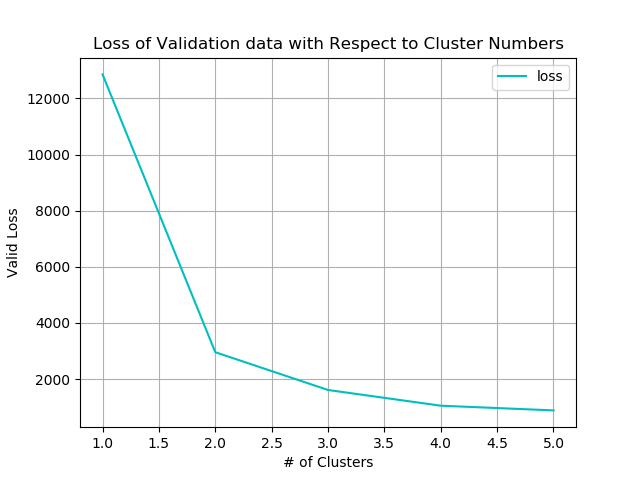
\includegraphics[width=.45\linewidth]{imgs/clusterNew.png}\hfill
  \caption{Change in validation loss with respect to cluster numbers}
  
\end{figure}





\section{Mixture of Gaussians} 
\subsection{The Gaussian cluster mode}
\subsubsection{Log Probability density function implementation}

\qquad Randomly initialize $K$ centers, we have: \begin{align*}
    \mathcal{N}(x|\mu_{k}, \sigma_k^2)) &= P( x|\mu_{k}, \sigma_k^2))\\
   log\mathcal{N}(x|\mu_{k}, \sigma_k^2))&=logP(x|\mu_{k}, \sigma_k^2)) \\
   &=log(\frac{1}{\sqrt{2\pi}\sigma_k}exp(\frac{-(x-\mu_k)^2}{2\sigma_k^2})) \\
   &= log(\frac{1}{\sqrt{2\pi}\sigma_k})+(\frac{-(x-\mu_k)^2}{2\sigma_k^2})
\end{align*}

Python implementation of above equation show below. 

 \lstinputlisting[language=python, caption = Log probability density]{functions/log_GaussPDF.py}

\subsubsection{Log Probability of the cluster variable z given data vector x}

\qquad Basic idea of this part is to invert the probability found in part 2.1.1. Apply Bayer's rule, we can simply get: 
\begin{align*}
    P(z = k|x) &= \frac{P(x|z = k)P(z= k)}{P(x)} \\
    &= \frac{P(x|z = k)P(z= k)}{\sum_i P(x|z = i)P(z= i)}
\end{align*}
\qquad Where in above equation, $\sum_{i=1}^{i=K}P(x|z = i)P(z= i)$ gives all possible scenarios of clustering. Therefore, 

\begin{align*}
    logP(z = k|x) &= logP(x|z = k)+logP(z = k) - log\sum_i exp(logP(x|z = i) + logP(z= i))
\end{align*}

 \lstinputlisting[language=python, caption = Log posterior clustering probability]{functions/log_posterior.py}


\subsection{Learning the MoG}
\subsubsection{}
\qquad The reasonable initial value for parameters were shown in Listing 4 below. We had enforced the constrict for $\pi$ by using a softmax function, and enforced $\sigma$ in the range of 0 to inf by doing exp to $\sigma$. All parameters were initialized by sampling from the standard normal distribution, with the standard deviation of $0.01$, and table 3 shows the reason for this selection. \\


\lstinputlisting[language=python, caption = Initialization of parameters.]{functions/initial.py}
% \begin{figure}[H]
% \centering

%   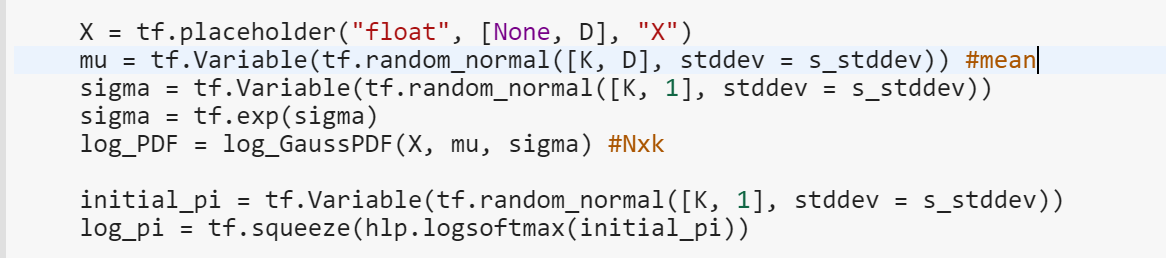
\includegraphics[width=.7\linewidth]{imgs/initial.PNG}
%   \caption{Initialization of parameters.}

% \end{figure}

\begin{table}[H]
\centering
{\small

\begin{tabular}{cccccc}
\hline
$\sigma $ & Beginning Loss      & Best Loss\\ \hline
0.01 & 49016.14  & 17132.400 \\ 
1 & 52995.58  & 17132.543 \\ 
10 & 359978000 & 82524.844\\ \hline
\end{tabular}
}
\vspace{-0.2cm}
\caption{Choice of standard deviation value when initializing parameters}
\label{tab:Number of hidden units}
\vspace{-0.4cm}
\end{table}

With these parameters and selection of $k=3$, $iteration=1000$. The result of trained test data had shown below. \\

\begin{figure}[H]
\centering

  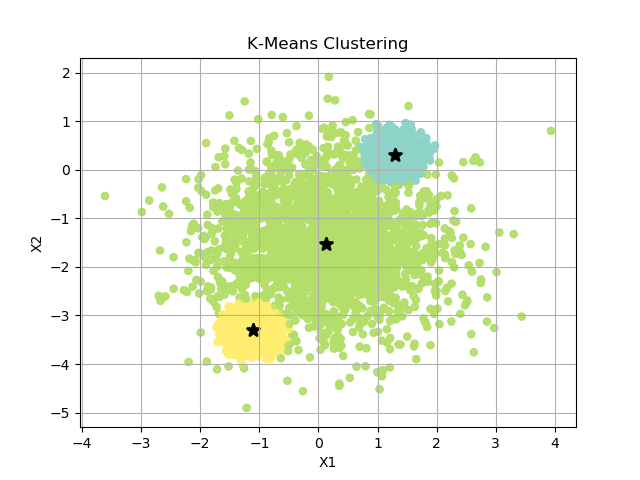
\includegraphics[width=.42\linewidth]{imgs/K_cluster_G.png}
  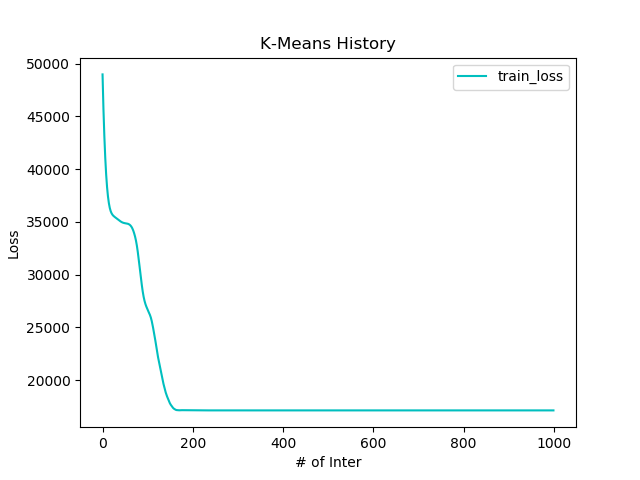
\includegraphics[width=.42\linewidth]{imgs/lossC.png}
  \caption{2D cluster plot and Test data loss when $K=3$.}

\end{figure}

\begin{table}[H]
\centering
{\small

\begin{tabular}{cccccc}
\hline
Cluster  & $\pi$      & Mean & $\sigma$\\ \hline
1 & -1.0983235  & [1.299 0.308] & 0.0388 \\ 
2 & -1.1029158   & [-1.101 -3.307] & 0.0391 \\ 
3 & -1.094615  & [0.106 -1.527] & 0.9872\\ \hline
\end{tabular}
}
\vspace{-0.2cm}
\caption{Best model parameters for test data set.}
\label{tab:Number of hidden units}
\vspace{-0.4cm}
\end{table}


\subsubsection{}
\qquad As shown in figure 10 below, the loss for validation data had decreased as k increases, however,the validation loss didn't have obvious decrease anymore from $k=3$ onward, therefore, 3 is the best choice of k.\\

\begin{figure}[H]
\centering
  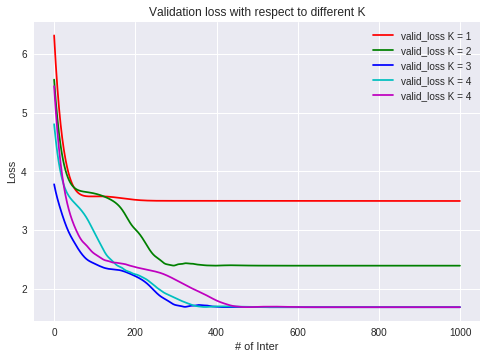
\includegraphics[width=.42\linewidth]{imgs/p2_2_2_loss.png}
  \caption{Validation loss with respect to different K.}
\end{figure}


\begin{figure}[H]
\centering
  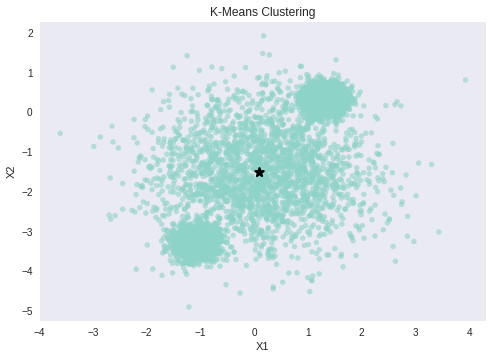
\includegraphics[width=.3\linewidth]{imgs/p2_2_2pK1.png}
  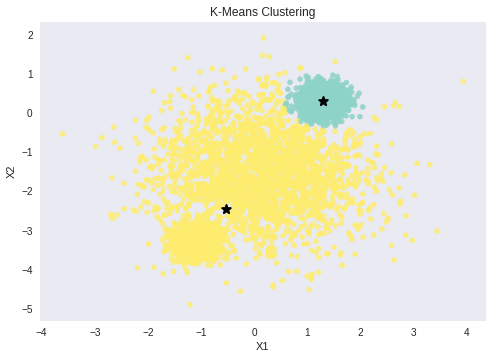
\includegraphics[width=.3\linewidth]{imgs/p2_2_2pK2.png}
  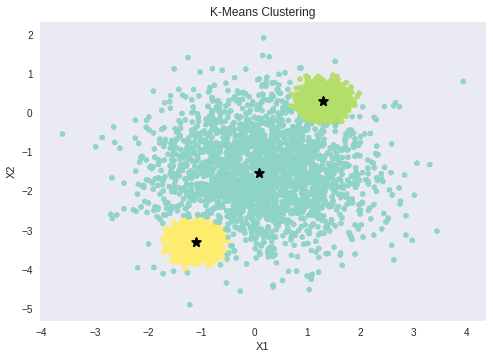
\includegraphics[width=.3\linewidth]{imgs/p2_2_2pK3.png} 
  \caption{Validation loss with respect to different K(K from 1 to 3).}
\end{figure}

\begin{figure}[H]
\centering
  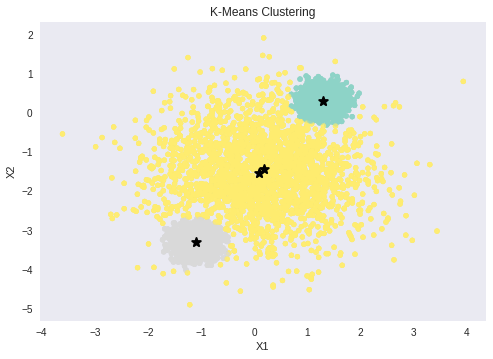
\includegraphics[width=.33\linewidth]{imgs/p2_2_2pK4.png}
  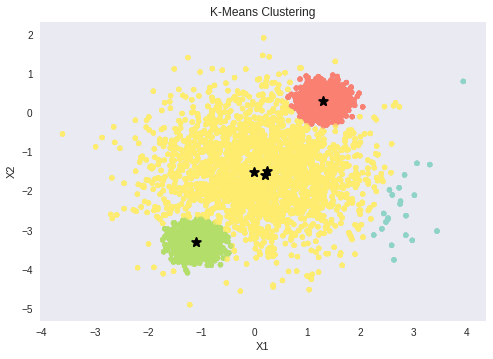
\includegraphics[width=.33\linewidth]{imgs/p2_2_2pK5.png}

  \caption{Validation loss with respect to different K(K from 4 to 5).}
\end{figure}

\subsubsection{}
\qquad Figure 12 had showed the validation loss with different K by using GMM (at right hand-side), the loss values for all K values were similar after 1000 iterations of training, however, there was a large increase in the decay of loss values from $K=5$ to $K=10$, after that, the decay of loss values had not been changed much. Therefore, $K=10$ is the reasonable amount of clusters for training using GMM.\\

In the other side, by looking at the loss values for different K values by using K-means, there was not large decrease after K=10, therefore, the reasonable amount of clusters is also 10. In addition, K-means didn't performed as well as GMM with high dimensional data.\\

\begin{table}[H]
\centering
{\small

\begin{tabular}{ccccccc}
\hline
Cluster K  & 5  & 10 & 15 & 20 & 25 & 30 \\ \hline
Final training loss using GMM & 50525.19  & 44320.33 & 44496.09 & 44057.45 & 44752.05 & 44147.00 \\
Final training loss using K-means & 247141.92  & 143545.07 & 143544.89 & 143545.48 & 143544.95 & 143544.96 \\\hline
\end{tabular}
}
\vspace{-0.2cm}
\caption{Final training loss with different K, $if\_valid = True$.}
\label{tab:Number of hidden units}
\vspace{-0.4cm}
\end{table}



\begin{figure}[H]
\centering

  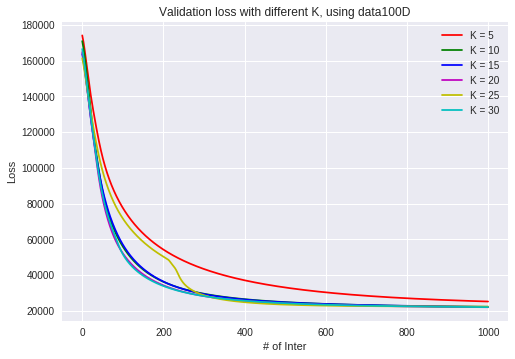
\includegraphics[width=.45\linewidth]{imgs/p2_2_3loss.png}
%   \caption{Validation loss, using GMM. }
  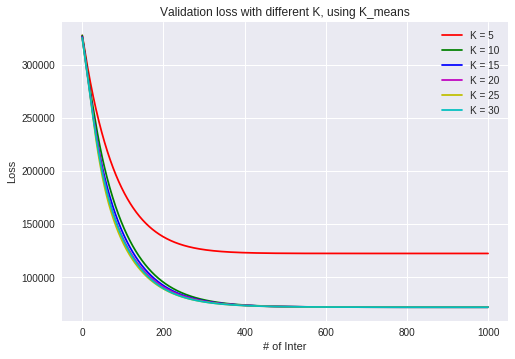
\includegraphics[width=.45\linewidth]{imgs/p2_2_3lossk.png}
  \caption{Validation loss, using GMM andK -means. }

\end{figure}



\end{document}
